\documentclass{sig-alternate}
\usepackage{subfigure}
\usepackage{graphicx}
\usepackage{url}

\clubpenalty=10000
\widowpenalty = 10000


\usepackage{amsmath,amssymb}
\usepackage{amstext}
\usepackage{dsfont}
\usepackage{xspace}
\usepackage{epsfig}
\usepackage{balance}
\usepackage[noend]{algorithmic}
\usepackage{algorithm}
\usepackage{color}
\usepackage{tikz}
\usetikzlibrary{calc}


\newtheorem{conjecture}{Conjecture}
\newtheorem{mutation}{Mutation Operator}
\newtheorem{definition}{Definition}
\newtheorem{theorem}{Theorem}
\newtheorem{lemma}{Lemma}
\newtheorem{corollary}{Corollary}
\newtheorem{claim}{Claim}

\renewcommand{\epsilon}{\varepsilon}
\newcommand{\R}{\mathds{R}}
\newcommand{\N}{\mathds{N}}
\newcommand{\Q}{\mathds{Q}}
\newcommand{\Z}{\mathds{Z}}

\begin{document}

\title{ComeTogether - an android app to meet new people}

\numberofauthors{2}
\author{
	\alignauthor Christof Ochmann\\
	\affaddr{University of Applied Sciences Zittau/G\"{o}rlitz}\\
	\affaddr{02826 G\"{o}rlitz, Germany}\\
	\email{sichochm@hs-zigr.de}\\
	\and
	\alignauthor Ingo K�rner\\
	\affaddr{University of Applied Sciences Zittau/G\"{o}rlitz}\\
	\affaddr{02826 G\"{o}rlitz, Germany}\\
	\email{siinkoer@hs-zigr.de}\\
}


\maketitle
\begin{abstract}
This work based on the document "Come-Together-App", which was created in Wirtschaftsinformatik II in a course of studies of tourism. The ideas of the project "Come-Together-App"  are realized as a prototype in "ComeTogether - an android app to meet new people". Both, frontend and backend are analysed, desgined and implemented.

\end{abstract}



\category{F.2.2}{Analysis of Algorithms and Problem Complexity}{Nonnumerical Algorithms and Problems}
\terms{Algorithms, Design, Performance, Theory}
\keywords{Parallel evolutionary algorithms, island model, spatial structures, offspring populations, runtime analysis}

\input{Ingo/Introduction}
\section{previous work}\label{sec:previouswork}
There are flirt apps for smartphones like "myamio - Die Partnersuche f�r das iPhone" which are used by singles to contact others. Beside flirt apps there are also calendar of events as app-download for enterprising people. A calender of event app is "PRINZ iPhone-App f�r Veranstaltungen, Bars und Clubs in Ihrer Stadt". This app is for people who mainly want to find a new locality or enterprise, independent of the people who take part. A certain link of calendar of events and flirt app provides the free "Barcardi Togethering App". In this app there is only the possibility to date your own facebook friends but you cannot meet strangers. In contrast to Barcardi app there is no need to join a social network to run ComeTogether app.
What can you do, if you are not interested in relationship and your friends have no time for you but you want to go out and meet some people or you are alone in an unfamiliar environment and want to have an enterprise?
The ComeTogether app is a new and modern way to contact people.
You can meet new people, share common interests and promote sociability.
ComeTogether can reduce barriers of single or lonely people which long for new people.
Moreover, the probability of a disappointment is less if you meet a person with same interests electronically first than you have a face-to-face encounter immediately.
And the electronically way has a certain distance to the unknown people and that gives more security.
ComeTogether is a completely new mixture of calender of events and dating app.
ComeTogether is not limited to a niche like dating apps, which are only made for singles.

\section{requirements engineering}\label{requirementsengineering}
Figure \ref{fig:useCaseDiagram} shows the use case diagram for ComeTogether.

\section{Design}\label{Design}

In figure \ref{fig:UserServiceREST} you can see the design for the UserService. UserServiceREST encapsulate the REST-Functionality of the UserService. UserPersistence access database with prepared statements p.e. to save, read or delete users. Between UserServiceREST and UserPersistence are service class and DAO class to encapsulate different levels of abstraction. Beside UserServiceREST there are the classes EventServiceREST, ParticipationServiceREST and MessageServiceREST. EventServiceREST in figure \ref{fig:EventServiceREST} creates, reads and deletes events. ParticipationServiceREST in figure \ref{fig:ParticipationServiceREST} creates participations and gives back a list of participation for a given eventid or a given userid. MessageServiceREST in figure \ref{fig:MessageServiceREST} creates, reads or deletes messages.

\begin{figure}[htp]
\centering
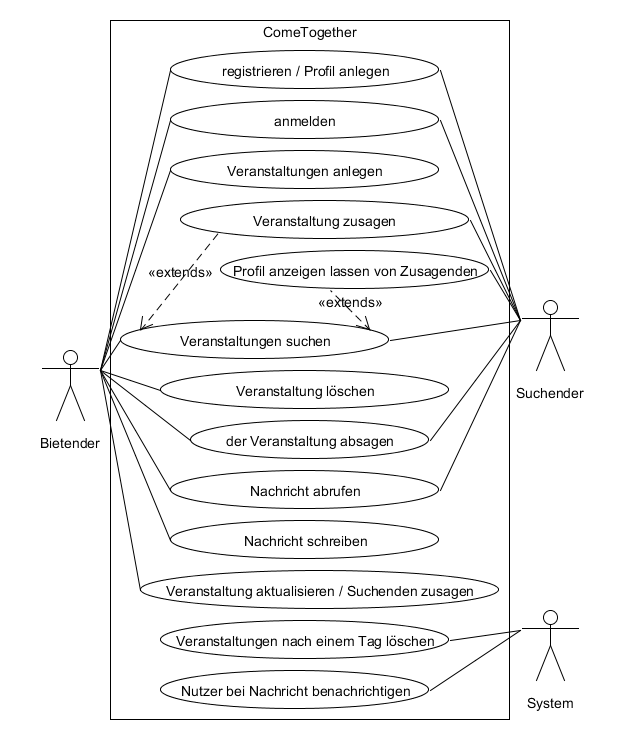
\includegraphics[width=0.5\textwidth]{Ingo/pictures/UseCaseDiagram.png}
\caption{use case diagram}
\label{fig:useCaseDiagram}
\end{figure}


\begin{figure}[htp]
\centering
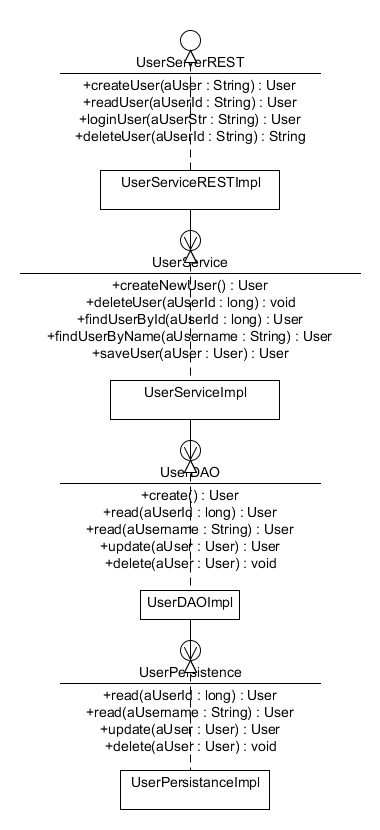
\includegraphics[width=0.5\textwidth]{Ingo/pictures/Design_User.png}
\caption{desing class diagramm UserServiceREST}
\label{fig:UserServiceREST}
\end{figure}


\begin{figure}[htp]
\centering
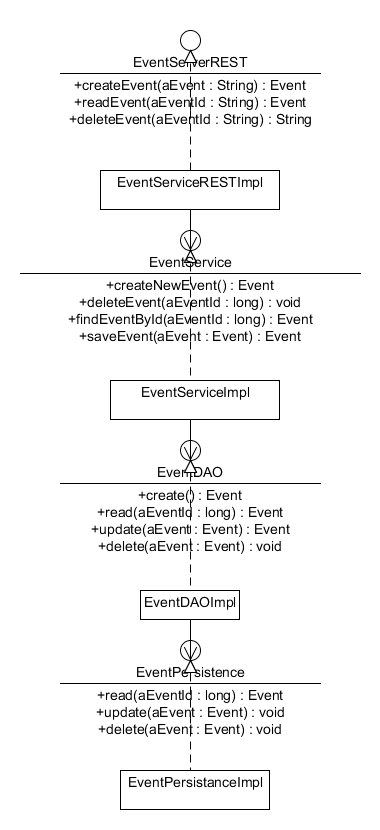
\includegraphics[width=0.5\textwidth]{Ingo/pictures/Design_Event.png}
\caption{desing class diagramm EventServiceREST}
\label{fig:EventServiceREST}
\end{figure}


\begin{figure}[htp]
\centering
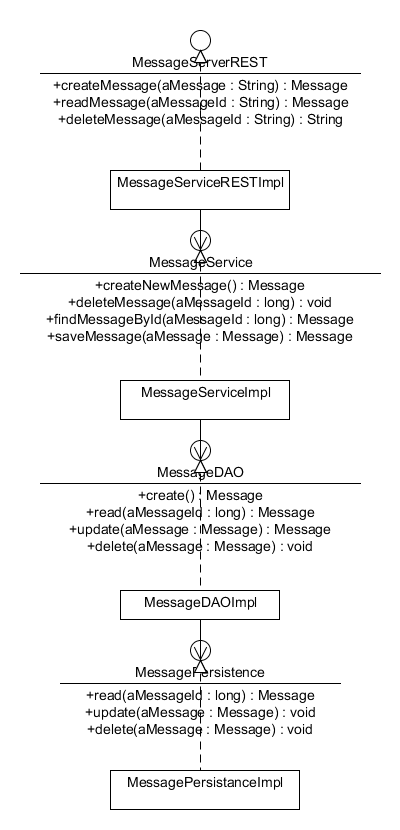
\includegraphics[width=0.5\textwidth]{Ingo/pictures/Design_Message.png}
\caption{desing class diagramm MessageServiceREST}
\label{fig:MessageServiceREST}
\end{figure}


\begin{figure}[htp]
\centering
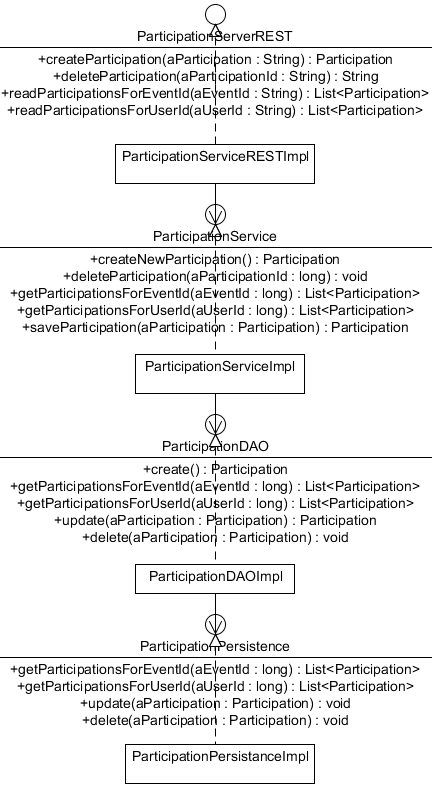
\includegraphics[width=0.5\textwidth]{Ingo/pictures/Design_Participation.png}
\caption{desing class diagramm ParticipationServiceREST}
\label{fig:ParticipationServiceREST}
\end{figure}

\section{database}\label{database}
In figure \ref{fig:EERdiagram} you can see the data base design of ComeTogether.

\begin{figure}[htp]
\centering
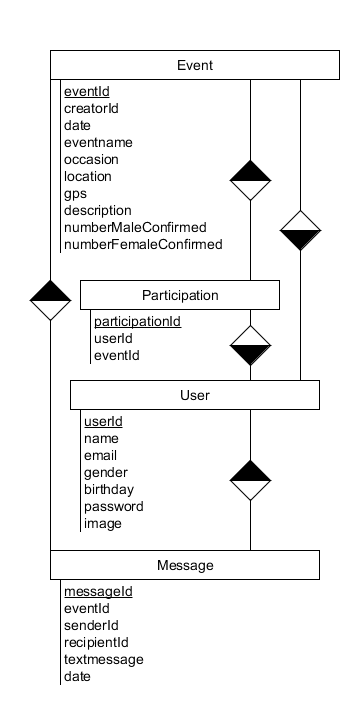
\includegraphics[width=0.5\textwidth]{Ingo/pictures/EER-diagram.png}
\caption{eer-diagram}
\label{fig:EERdiagram}
\end{figure}


\section{Preliminaries}
\label{sec:Preliminaries}

\section{Previous Work}
\label{sec:PreviousWork}


\section{Sorting}
\label{sec:Sorting}

...


\section{Shortest Paths}
\label{sec:ShortestPaths}


...


\section{Eulerian Cycles}
\label{sec:EulerianCycles}

...

\subsection{Edge Walks}

...

\subsection{Restricted Mutation Operators}

...

\subsection{Adjacency List Matchings}

...

\section{Conclusions}
\label{sec:Conclusions}


\subsection*{Acknowledgments}
The authors would like to thank .....the German fast food industry for keeping us alive.

\bibliographystyle{abbrv}
\bibliography{literature-short}
\balance

\end{document}
